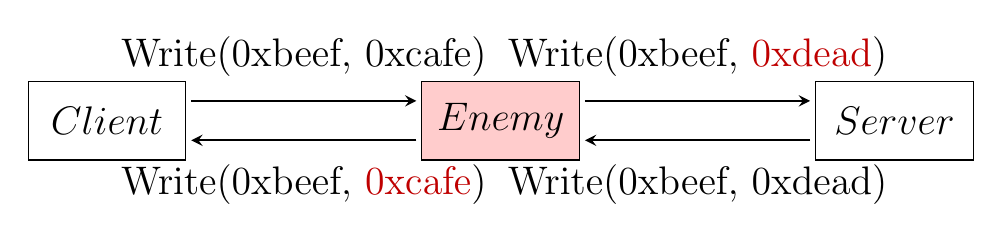
\begin{tikzpicture}[font=\Large,
    arrow/.style={thick,->,shorten >=2pt,shorten <=2pt,>=stealth},
]
    \draw (0,0) rectangle (2,1) node [pos=.5] {$Client$};
    \draw[fill=red!20!white] (5,0) rectangle (7,1) node [pos=.5] {$Enemy$};
    \draw (10,0) rectangle (12,1) node [pos=.5] {$Server$};

    % Clients - Servers links
    \draw[arrow] (2,.75) -- (5,.75)  node [anchor=south, pos=.5, align=center, above=.5em] {Write(0xbeef, 0xcafe)};
    \draw[arrow] (7,.75) -- (10,.75) node [anchor=south, pos=.5, align=center, above=.5em] {Write(0xbeef, {\color{red!75!black} 0xdead})};
    \draw[arrow] (10,.25) -- (7,.25)   node [anchor=north, pos=.5, align=center, below=.5em] {Write(0xbeef, 0xdead)};
    \draw[arrow] (5,.25) -- (2,.25)    node [anchor=north, pos=.5, align=center, below=.5em] {Write(0xbeef, {\color{red!75!black} 0xcafe})};
\end{tikzpicture}
